\documentclass[11pt,a4paper]{article}
\usepackage[margin=2.5cm]{geometry}
\usepackage[T1]{fontenc}
\usepackage{lmodern,microtype,graphicx,booktabs,amsmath,xcolor,framed,hyperref}
\hypersetup{colorlinks,linkcolor=black,citecolor=black,urlcolor=blue!50!black}
\definecolor{todo}{rgb}{0.85,0.25,0.15}
% Sections in red boxes are for the author to write in his own words.
% Delete each box once its section is written.
\newenvironment{authorbox}[1]{\begin{framed}\noindent\textcolor{todo}{\textbf{Author to write: #1}}\par\small}{\end{framed}}

\title{How many pixels does a coarsening exponent need?\\[4pt]
\large Resolution bias in growth exponents fitted from two-phase images}
\author{Django Thompson\\ \small Independent researcher, Oxford, UK}
\date{Preprint, \today}

\begin{document}
\maketitle

\section*{Abstract}
\begin{authorbox}{abstract (about 150 words)}
One sentence each: why growth exponents are fitted from images; the question
(how coarse can an image be before the fitted exponent is biased); what was
done (simulations with a known answer, blind tests on two public X-ray
datasets, a printed-tile camera test); the main numbers (about 0.05--0.07 too
low at $\sim$0.7 pixels per domain, under 0.01 above about two); the practical
rule; and that a published static criterion already protects against it.
\end{authorbox}

\section{Introduction}
\begin{authorbox}{introduction (400--600 words)}
\begin{itemize}
\item Coarsening and why $L\propto t^n$ matters: LSW gives $n=1/3$ for bulk
diffusion \cite{lifshitz1961,wagner1961}; $1/4$ and $1/5$ point to other paths.
Exponents are used to identify mechanisms and predict service ageing.
\item Exponents are fitted from micrographs taken at one magnification, so
early images have the smallest features in pixels.
\item What is known: resolution distorts image statistics
\cite{ledesma2018,zabler2007}; practical rules discard small features
\cite{werz2014}; two-point correlations have described coarsening in the same
Al--Cu data used here \cite{sun2017}.
\item The gap: how large the error becomes in a fitted exponent, and whether
the usual fit checks reveal it.
\item Your route into the question (EPQ on entropy and the arrow of time) in one
or two sentences, if you want it.
\end{itemize}
\end{authorbox}

\section{Methods}
\subsection{Simulations}
A binary alloy is represented by the two-dimensional Ising lattice gas on a
$128\times128$ periodic square lattice. Dynamics conserve composition: the only
move swaps two neighbouring sites, accepted with the Metropolis rule
\cite{kawasaki1966,metropolis1953}. Each run starts from a random configuration
and is quenched to $0.65\,T_c$. Time is counted in Monte Carlo sweeps (one
attempted move per site). Two compositions were simulated, 50:50 and 15:85.
Thirty-two development trajectories (16 per composition) were used while the
analysis was designed, and 16 further trajectories with new seeds (8 per
composition) were held out and analysed with the analysis fixed. In two
dimensions this model approaches $n=1/3$ only slowly \cite{huse1986}; over the
fit window used here the median native exponents are 0.229--0.244. The
reference for every comparison is therefore each trajectory's own
full-resolution exponent, not $1/3$.

\subsection{Images and the coarse camera}
At each recorded time the full-resolution configuration is the true image. A
coarser camera is modelled by averaging $k\times k$ blocks of sites ($k=2,4,8$)
and thresholding the block means at zero, with exact ties assigned to the
$+1$ phase. Blur and noise were studied separately in real images
(Section~\ref{sec:real}).

\subsection{Length and exponent}
The domain length is the two-point correlation length: for each axis, the
normalised correlation of the mean-subtracted image is computed with linear
(non-wrapping) pair counting, and the length is the interpolated distance at
which it first falls to $1/2$. The horizontal and vertical values are
averaged. Pixels per domain is this length divided by the pixel size. The
exponent $n$ is the least-squares slope of $\ln L$ against $\ln t$ over
1{,}000--20{,}000 sweeps (24 snapshots). The error at resolution $k$ is
$n_k-n_1$ for the same trajectory.

\section{Results}
\subsection{Simulated images}
Figure~\ref{fig:example} shows one snapshot at full resolution and after
$2\times$ and $4\times$ coarsening. Table~\ref{tab:errors} and
Figure~\ref{fig:error} give the exponent error for every trajectory. Near 1.2
pixels per domain ($2\times$) the median error was $-0.005$ at 50:50 and
$-0.011$ at 15:85. Near 0.65 pixels per domain ($4\times$) it was $-0.057$ and
$-0.073$, and near 0.47 ($8\times$) $-0.16$ and $-0.22$. Every coarsened fit
read too slow. The held-out trajectories reproduced the development medians to
within 0.006.

Which step of the coarse camera causes the error depends on the coarsening.
Measuring the block-averaged grey image directly, without thresholding, gave a
median error of about $-0.036$ at $2\times$ but about $-0.001$ at $4\times$ for
50:50, so neither averaging nor thresholding is responsible in general
(last column of Table~\ref{tab:errors}).

\begin{figure}[t]\centering
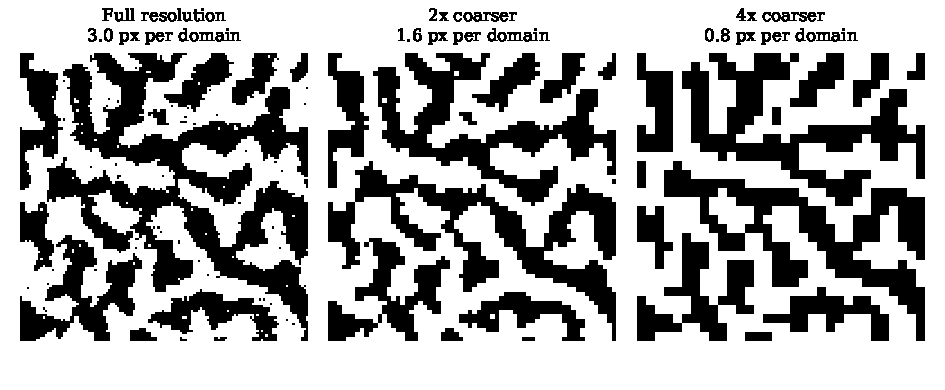
\includegraphics[width=\linewidth]{figures/fig1_coarsening.pdf}
\caption{One 50:50 configuration at 10{,}600 sweeps, at full resolution and
after $2\times$ and $4\times$ block averaging and thresholding. Pixels per
domain is the correlation length divided by the pixel size.}
\label{fig:example}
\end{figure}

\begin{table}[t]\centering\small
\caption{Exponent error $n_k-n_1$ by coarsening factor $k$. Pixels per domain is
the median over the fit window. The last column measures the block-averaged
grey image without thresholding.}
\label{tab:errors}
\begin{tabular}{llrrrrr}
\toprule
Set & Composition & $k$ & Px/domain & Median error & Range & Averaging only\\
\midrule
\csname @@input\endcsname results/table_errors.tex
\bottomrule
\end{tabular}
\end{table}

\begin{figure}[t]\centering
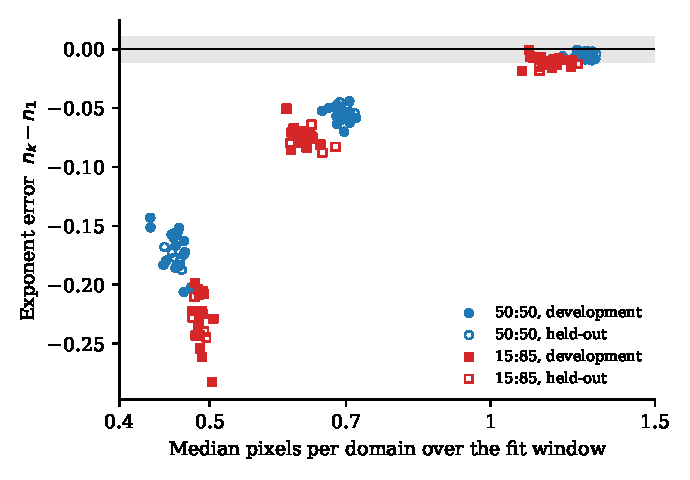
\includegraphics[width=.72\linewidth]{figures/fig2_error_vs_pixels.pdf}
\caption{Exponent error against median pixels per domain for every
trajectory and coarsening factor. Filled: development; open: held-out. The
grey band marks $\pm0.01$.}
\label{fig:error}
\end{figure}

\subsection{Real images}\label{sec:real}
\begin{authorbox}{real-image results, with their data and code pushed first}
\begin{itemize}
\item Al--Ge tomography \cite{fell2023}, four ageing times, followed over time:
errors by pixels per domain; the single-image check overstated the error here.
\item Al--Cu semi-solid tomography \cite{gibbs2016}, blind test with rules
written before download: errors by pixels per domain; both slicing directions.
\item Blur and noise added to both datasets.
\item Printed-tile camera test: real optics and blind (Otsu \cite{otsu1979})
thresholding against a known answer. Report against the committed protocol.
\end{itemize}
The November numbers in the outreach brief are not yet reproducible from the
repository. Push the analysis and its outputs, then quote them here.
\end{authorbox}

\subsection{A screen for at-risk fits}
Coarsening an image series by a further factor of two and refitting gives a
warning signal $n_{2k}-n_k$. On the held-out trajectories
(Figure~\ref{fig:screen}), a warning larger than 0.01 in magnitude flagged all
22 fits whose true error exceeded 0.01, but also 16 of the 26 fits whose error
did not. Warning and true error were strongly correlated ($r=0.96$ for
coarsened images), with the warning typically two to three times larger. It
is a sensitive but unspecific screen, and is implemented with this caveat in
an in-browser tool (Data availability).

\begin{figure}[t]\centering
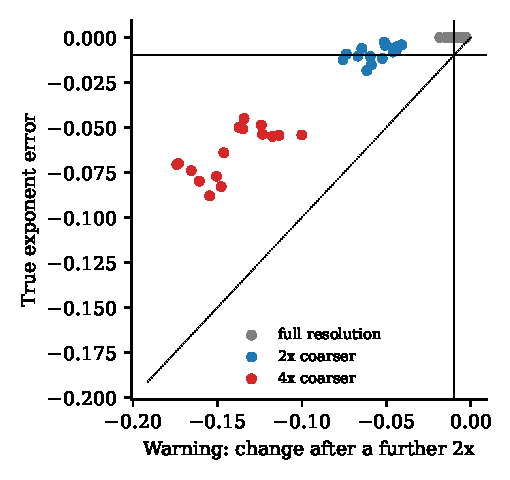
\includegraphics[width=.5\linewidth]{figures/fig3_screen.pdf}
\caption{The $2\times$ warning against the true exponent error on held-out
trajectories. Lines mark $\pm0.01$; the dotted line is equality.}
\label{fig:screen}
\end{figure}

\section{Discussion}
\begin{authorbox}{discussion (400--600 words)}
\begin{itemize}
\item Size of the effect in context: the gap between $1/3$ and $1/4$ is 0.083.
\item Relation to the published criterion \cite{ledesma2018}: did it protect
exponents in your tests, and what does that mean for the contribution?
\item Why the usual fit checks miss the bias, if your November data show it.
\item The practical rule: about two pixels per domain for sharp images, three
or more with blur; earliest images are the ones at risk.
\item What would change your mind; what an SEM ageing series would test.
\end{itemize}
\end{authorbox}

\section{Limitations}
The simulations are two-dimensional, sharp-edged and uncalibrated to any alloy,
at one temperature in the results shown. Real-image tests use 2D slices of two
public tomography datasets, neither of them SEM, with few time points. The
coarse camera is a model; its fidelity to real detectors is tested only by the
printed-tile experiment. No laboratory has validated the screen or the tool.

\section*{Data and code availability}
All simulation code, archived trajectories, analysis scripts and this paper's
figure script (\texttt{paper/make\_figures.py}) are at
\url{https://github.com/djangothompson12-alt/ising-monte-carlo}. The
in-browser Pixel check is in \texttt{tools/pixel\_check}.

\section*{Use of AI tools}
\begin{authorbox}{check and finalise}
AI assistants wrote most of the simulation and analysis code, proposed many of
the specific tests, drafted the methods and results text of this preprint from
the archived results, and checked references. The author chose the question,
set the pass/fail rules before each test, checked the results, and wrote the
abstract, introduction and discussion. A full record is in
\texttt{AI\_USE\_AND\_CONTRIBUTIONS.md}.
\end{authorbox}

\begin{thebibliography}{99}\small
\bibitem{lifshitz1961} I.~M. Lifshitz and V.~V. Slyozov, J. Phys. Chem. Solids \textbf{19}, 35 (1961).
\bibitem{wagner1961} C.~Wagner, Z. Elektrochem. \textbf{65}, 581 (1961).
\bibitem{huse1986} D.~A. Huse, Phys. Rev. B \textbf{34}, 7845 (1986).
\bibitem{kawasaki1966} K.~Kawasaki, Phys. Rev. \textbf{145}, 224 (1966).
\bibitem{metropolis1953} N.~Metropolis \emph{et al.}, J. Chem. Phys. \textbf{21}, 1087 (1953).
\bibitem{ledesma2018} R.~Ledesma-Alonso \emph{et al.}, Phys. Rev. E \textbf{97}, 023304 (2018).
\bibitem{zabler2007} S.~Zabler \emph{et al.}, Acta Mater., doi:10.1016/j.actamat.2007.05.028 (2007).
\bibitem{werz2014} T.~Werz \emph{et al.}, Mater. Charact. \textbf{90}, 185 (2014).
\bibitem{sun2017} Y.~Sun, A.~Cecen, J.~W. Gibbs, S.~R. Kalidindi and P.~W. Voorhees, Acta Mater. \textbf{132}, 374 (2017).
\bibitem{otsu1979} N.~Otsu, IEEE Trans. Syst. Man Cybern. \textbf{9}, 62 (1979).
\bibitem{fell2023} J.~Fell, Segmented X-ray tomography of solid-state-aged Al--Ge, Mendeley Data, doi:10.17632/hj9njz3rxp.1 (2023).
\bibitem{gibbs2016} J.~W. Gibbs, P.~W. Voorhees and J.~L. Fife, Liquid--solid metallic mixture coarsening data, Materials Data Facility, doi:10.18126/M2CC73.
\end{thebibliography}
\end{document}
